\section{準備}
本章では,本論において核となる技術内容・特徴およびそのメカニズムについて説明する.
\subsection{DNS プロトコル}
\label{sec:dns-protocol}
DNS(Domain Name System)は,インターネットに接続された無数のコンピュータを一意に識別するためのIPアドレスを,人が認識しやすいドメイン名に変換するシステムである.
元来,インターネット上でのホストの識別にはIPアドレスが使用されてきた.
しかし,32bitの名前空間で10進数表記のIPv4(E.g. ``192.168.0.1")や128bitの名前空間で16進数表記のIPv6(E.g. ``2001:200:16a:8::230")は,決して人にとって認識しやすいものではない.
そこで,自然言語のようにアルファベットや数字で表記されるホスト名とIPアドレスを関連づける仕組みが登場した.
当初,hosts.txtと呼ばれる対応表は,中央集権的に管理されていた.
しかし,ホスト数の増大に伴い,管理が困難になっていく.
その解決策として登場したのが,管理するドメインをゾーンで切り出し権限を委譲していく分散的な階層構造を持つDNSである.

DNSのシステムアーキテクチャは,クライアント・サーバ構成で成り立っている.
一般に,クライアントがドメインを問い合わせた場合,サーバはドメインに対応づけているIPアドレスを応答することで,クライアントはドメインに対応づけられたIPアドレスを解決することができる.
%ドメインからIPアドレスの解決は正引きと呼ばれ,IPアドレスからドメインの解決を逆引きと呼ぶ.

\subsubsection{ドメイン}
ドメインは,数字とアルファベットおよびハイフン(``-")の文字列で表記され,最大長は63オクテットと定義される.
また,ドメインはルートを頂点とする階層構造で構成され,各階層にはドメインを管理する主体として権威サーバが存在し,管理主体を委譲していくことによって分散的にデータベースを管理する仕組みで動作する.

\begin{figure}[h]
 \centering
 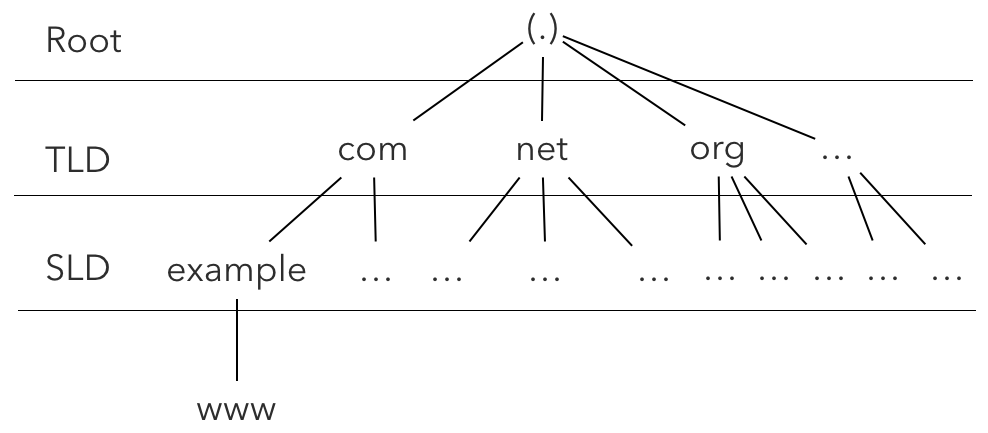
\includegraphics[width=12.0cm]{figure/dns-architecture.png}
 \caption{ドメインの名前空間}
 \label{fig:dns-architecture}
\end{figure}

ドメイン名は,ドメインに相当するラベルをドット区切りで表され,最大長は255オクテットである.
ドメイン名は右から順に階層序列が表現され,ドットで表現されるルートは一般には省略される.
最も右に位置づくラベルがTLD(Top Level Domain)であり,そのTLDからn番目(n $\mid$ n $\in$ $\mathbb{N}$)のラベルが第 n レベルドメインである.

TLDを大別すると,``.com"や``.net"をはじめとした特定分野別のgTLD(global Top Level Domain),``.jp"や``.ch"のような国ごとに割り当てられているccTLD(Co\\untry Code Top Level Domain)の二つに分けられる.

%TLDごとに登録するプロセスや必要書類,金額は異なり,上いの

\subsubsection{サービスの種類}
DNSのサービスは,機能に応じて3つに分けられる.
\begin{itemize}
 \item Stab Resolver
 \vspace{-3mm}
 \item Full Service Resolver
 \vspace{-3mm}
 \item Authorization Server
\end{itemize}

スタブリゾルバは,名前解決の問い合わせるを依頼するクライアントノードである.
フルサービスリゾルバ(キャッシュサーバ・リカーシブサーバとも呼称される)は,スタブリゾルバからの名前解決問い合わせをハンドリングするノードである.
過去に問い合わせられた情報をキャッシュとして保持する機能と,レコード情報を保持・提供する権威サーバに対する再帰問い合わせを行う機能を担う.
一般に,フルサービスリゾルバは,``root.hints"というルート権威サーバとそのアドレスが対応づけられたファイルを保持しており,再帰問い合わせの際にはこのファイルに基づき,最初の宛先となる権威サーバのアドレスを解決する.
権威サーバは,レコード情報を保持するサーバノードであり,フルリゾルバからの転送される問い合わせ依頼に応答する.

\subsubsection{リソースレコード}
ドメイン名に関連づけられる情報は,リソースレコード(Resorce Record, RR)と呼ばれる.
リソースレコードは,タイプが定義されており,目的ごとに使用されるタイプが異なる.
最も一般的なレコード,Aレコードタイプは,ドメインに対してIPv4アドレスを関連づけるために使用される.
名前解決において,クライアントはドメイン名とそのドメインに関連づけられたリソースレコードを指定する.
これによって,クライアントは,ドメインに関連づけられたリソースレコード情報を取得することができる.
表~\ref{tab:resource-record}は,主要なリソースレコードである.
\begin{table}[htb]
 \centering
  \begin{tabular}{ccc}
    \toprule
		\textbf{タイプ} & \textbf{値} & \textbf{意味} \\
    \midrule
    A & 1 &  ホストのIPv4アドレス \\
    NS & 2 & 権威サーバ \\
    MF & 4 & メール転送サーバ \\
    CNAME & 5 & 別名 \\
    SOA & 6 & 権威ゾーンの開始 \\
    NULL & 10 & NULL(実験用) \\
    PTR & 12 & ドメイン名のポインター(逆引き) \\
    HINFO & 13 & ホスト情報 \\
    MINFO & 14 & メールボックスおよびメールリスト情報 \\
    MX & 15 & メール交換 \\
    TXT & 16 & 任意文字列 \\
    \bottomrule
  \end{tabular}
 \caption{主要リソースレコード一覧}
 \label{tab:resource-record}
\end{table}


%リソースレコードのタイプごとの使用頻度を知りたい

\subsubsection{名前解決}
いま,クライアントから``www.example.com"のIPv4アドレスについて問い合わせられたとする.
はじめに,クライアントであるスタブリゾルバは,スタブリゾルバと同一セグメント内のフルサービスリゾルバもしくは,ネットワークセグメントに依らずインターネット上のどのクライアントからもアクセスできるパブリックなフルサービスリゾルバ(オープンリゾルバ,パブリックリゾルバとも呼称される)に問い合わせる.
フルサービスリゾルバははじめに,ドメイン名が``www.example.com"で,リソースレコードが``A"の応答レコードがキャッシュにあるかどうかを判別する.
キャッシュにヒットした場合にはキャッシュの情報をクライアントに応答され,ヒットしなかった場合には,root.hintsファイルを参照しルート権威サーバにリクエストパケットを転送する.
クエリ(問い合わせ)を受け取ったルート権威サーバは,ルートゾーン内の``com"ドメインが委譲された権威サーバのアドレスを応答する.
次に,フルサービスリゾルバは,``com"ドメインが委譲された権威サーバに対し同様のクエリを転送する.
``com"ドメインを管理する権威サーバは,同様にして,``com"ゾーン内の``example.com"が委譲された権威サーバのアドレスを応答する.
フルリゾルバは,``example.com"ドメインを委譲された権威サーバ宛に同様のクエリを転送する.
``example.com"ゾーンを管理する権威サーバは,保持するゾーンファイルからクエリされたドメインのリソースレコードについて探索し,探索の結果としてレコード情報をフルサービスリゾルバに応答する.
フルサービスリゾルバは,権威サーバからの応答されたレコード情報のTTL(Time To Live)の期間レコード情報をキャッシュしたのち,クライアントのスタブリゾルバに結果を応答する.
このようにして,再帰的な問い合わせの仕組みに基づき名前解決がとり行われる.

\newpage
\begin{figure}[h]
 \centering
 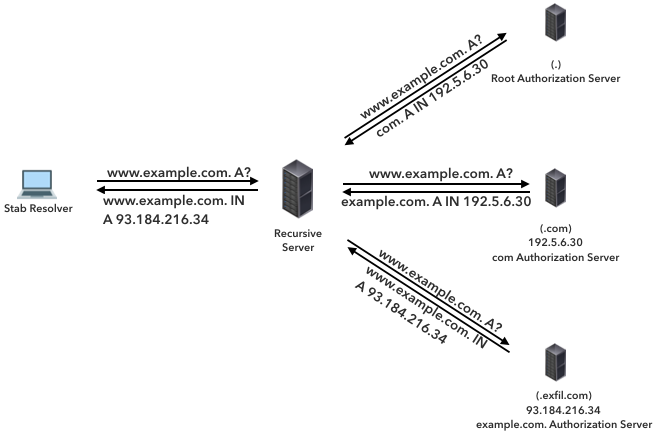
\includegraphics[width=12.0cm]{figure/dns-name-resolution.png}
 \caption{DNSによる名前解決}
 \label{fig:dns-name-resolution}
\end{figure}

\subsection{DNS Tunneling}
DNS Tunnelingは,
DNSは,\ref{sec:dns-protocol}節で示すように,ドメイン名とそのドメインに関連づけられたリソースレコードを解決するシステムである.
現在のインターネットにおいては,極めて重要な機能を担うプロトコルスタックの一つである.
他方で,本来
他方,クライアントサーバのアーキテクチャに基づき,スタブリゾルバの問い合わせ情報が権威サーバに直接転送される仕組みは,データ転送の仕組みでもある.
これによって,

\subsubsection{流出メソッド : DNS Exfiltration}
\label{sec:dns-exfiltration}
DNSを利用して情報を外部に転送するには,初めにデータの宛先となるドメイン(E.g. exfil.com)を作成することになる.
転送する際のキャリアとなるDNSクエリのラベルには,使用できる文字列は数字・アルファベット・ハイフン(``-")である必要があるため,一般にBase32・64を用いて転送したい情報をエンコーディングすることでこの制約条件を満たす.
用意できたQNAME(E.g. arbitrary-string.exfil.com)について,例えばAのリソースレコードをクエリすると,サブドメインの存在の有無に関わらず,宛先となるドメイン(exfil.com)に任意の情報を転送することができるという具合である.
このようにして,DNSをの名前解決の仕組みを応用することで,任意の権威サーバに任意の文字列を転送することができる.
以下\ref{fig:dns-exfiltration}に,DNS Exfiltrationのメカニズムについて図解する.

\begin{figure}[h]
 \centering
 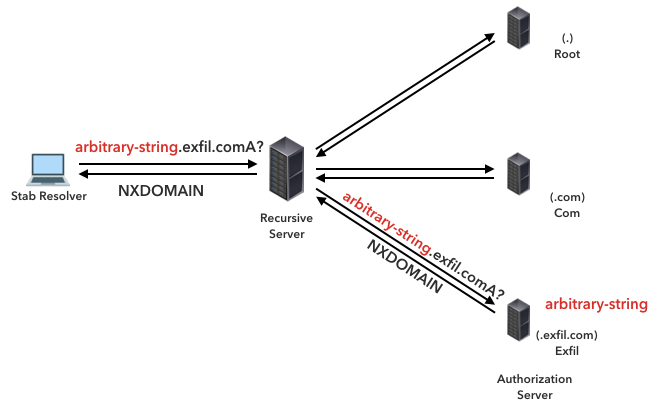
\includegraphics[width=12.0cm]{figure/dns-exfiltration.png}
 \caption{arbitrary-stringという任意の文字列が,DNSクエリのラベル部を用いて,事前に用意した権威サーバ(exfil.com)に転送される様子}
 \label{fig:dns-exfiltration}
\end{figure}

%1998年4月,DNS Tunnelingの手法は,NmapのBugtraqメーリングリストにて初めて公になったとされている\cite{bugtraq}.

\subsubsection{流入メソッド : DNS Infiltration}
DNS Infiltrationは,
管理する権威サーバのドメインに適当なホスト名(E.g. www)を作成し,そのホスト名のリソースレコード(E.g. TXT)に情報を付与していた場合には,そのホストへの問い合わせを通じて逆方向,すなわち権威サーバから任意の情報を転送することができる.
DNSのリソースレコードを転送キャリアとする流入通信のメカニズムを図解した様子が,\ref{fig:dns-infiltration}である.

\begin{figure}[h]
 \centering
 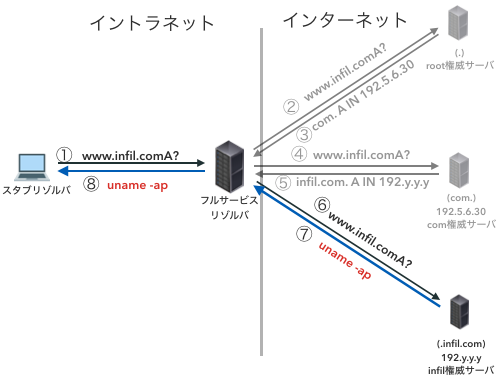
\includegraphics[width=10.0cm]{figure/dns-infiltration.png}
 \caption{事前にTXTレコードに登録された情報を問い合わせることで,権威サーバからの命令情報を取得している様子}
 \label{fig:dns-infiltration}
\end{figure}

このようにして,ExiltrationとInfiltrationメソッドを使うことで,データを送受信することができる.

%%\subsubsection{その他課題}
%%\subsection{秘匿通信}
%%秘匿通信(英Covert Channel)とは,
%%情報転送を実現するにあたり,データの転送を本来の設計としていないプロトコルにそのデータを注入する手法である.
%%\subsubsection{ステガノグラフィ}
%%\subsubsection{代替プロトコル}
%\subsection{分散ハッシュテーブル}
%\subsubsection{アルゴリズム}
%\subsubsection{暗号学的ハッシュ関数}
%\subsection{P2P}
%\subsubsection{アーキテクチャ}
